\documentclass[usenames,dvipsnames]{beamer}
\usepackage[utf8]{inputenc}
\usepackage[T1]{fontenc}

% \definecolor{custom_colour}{RGB}{65, 167, 241} % custom colour

\mode<presentation> {
\usetheme{Madrid} % there are a lot of different themes
% \usecolortheme{seahorse} % there are a lot of different colour themes
% \usecolortheme[named=custom_colour]{structure} % custom colour

% \setbeamertemplate{footline} % Custom footline
% {
%   \leavevmode%
%   \hbox{%
%   \begin{beamercolorbox}[wd=.333333\paperwidth,ht=2.25ex,dp=1ex,center]{author in head/foot}%
%     \usebeamerfont{author in head/foot}\insertshortauthor\hspace*{1ex}(\insertshortinstitute)
%   \end{beamercolorbox}%
%   \begin{beamercolorbox}[wd=.333333\paperwidth,ht=2.25ex,dp=1ex,center]{title in head/foot}%
%     \usebeamerfont{title in head/foot}\insertshorttitle
%   \end{beamercolorbox}%
%   \begin{beamercolorbox}[wd=.333333\paperwidth,ht=2.25ex,dp=1ex,right]{date in head/foot}%
%     \usebeamerfont{date in head/foot}\insertshortdate{}\hspace*{2em}
%     \insertpagenumber{} / \inserttotalframenumber\hspace*{2ex}
%   \end{beamercolorbox}}%
%   \vskip0pt%
% }
% \setbeamertemplate{footline} % To remove the footer line in all slides uncomment this line
% \setbeamertemplate{footline}[page number] % To replace the footer line in all slides with a simple slide count uncomment this line

% \setbeamertemplate{navigation symbols}{} % To remove the navigation symbols from the bottom of all slides uncomment this line
}

\usepackage{graphicx}

\usepackage{booktabs}

\usepackage{tikz}
\usetikzlibrary{positioning, fit, shapes}

\title[Short title]{Main Topic } % The short title appears at the bottom of every slide, the full title is only on the title page

\author{John Smith}
\institute[UCLA]
{
University of California \\
\medskip
\textit{john@smith.com}
}
\date{\today}

% \logo{\includegraphics[height=1.5cm]{lion-logo.png}}



\begin{document}

\begin{frame}
\titlepage
\end{frame}



\begin{frame}
\frametitle{Overview}
\tableofcontents
\end{frame}



\section{First Section}

\subsection{Subsection Example}

\begin{frame}
\frametitle{Paragraphs of Text}
Sed iaculis dapibus gravida. Morbi sed tortor erat, nec interdum arcu. Sed id lorem lectus. Quisque viverra augue id sem ornare non aliquam nibh tristique. Aenean in ligula nisl. Nulla sed tellus ipsum. Donec vestibulum ligula non lorem vulputate fermentum accumsan neque mollis.
\end{frame}

\begin{frame}
\frametitle{Multislide}
Line 1
\pause

Line 2
\pause
\end{frame}

\begin{frame}
\frametitle{Node multislide}
\onslide<+->{
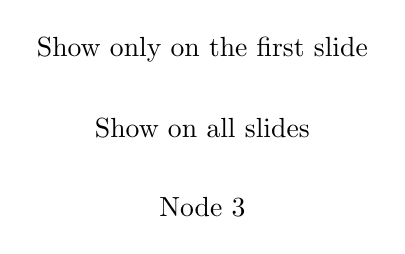
\begin{tikzpicture}
\node<1>[rectangle](node_1) at (0,0) {Show only on the first slide};
\node[rectangle](node_2) at (0,-1) {Show on all slides};
\onslide<+->{
\node[rectangle](node_3) at (0,-2) {Node 3};
}
\end{tikzpicture}
}
\end{frame}



\begin{frame}
\frametitle{Bullet Points}
\begin{itemize}
\item Bullet point
\end{itemize}
\end{frame}



\begin{frame}
\frametitle{Blocks of Highlighted Text}
\begin{block}{Block 1}
Lorem ipsum dolor sit amet, consectetur adipiscing elit. Integer lectus nisl, ultricies in feugiat rutrum, porttitor sit amet augue. Aliquam ut tortor mauris. Sed volutpat ante purus, quis accumsan dolor.
\end{block}
\end{frame}



\begin{frame}
\frametitle{Multiple Columns}
\begin{columns}[c] % The "c" option specifies centered vertical alignment while the "t" option is used for top vertical alignment

\column{.45\textwidth}
\textbf{Heading}
\begin{enumerate}
\item Statement
\item Explanation
\item Example
\end{enumerate}

\column{.5\textwidth} % Right column and width
Lorem ipsum dolor sit amet, consectetur adipiscing elit. Integer lectus nisl, ultricies in feugiat rutrum, porttitor sit amet augue. Aliquam ut tortor mauris. Sed volutpat ante purus, quis accumsan dolor.

\end{columns}
\end{frame}



\section{Second Section}

\begin{frame}
\frametitle{Table}
\begin{table}
\begin{tabular}{l l l}
\toprule
\textbf{Treatments} & \textbf{Response 1} & \textbf{Response 2}\\
\midrule
Treatment 1 & 0.0003262 & 0.562 \\
Treatment 2 & 0.0015681 & 0.910 \\
Treatment 3 & 0.0009271 & 0.296 \\
\bottomrule
\end{tabular}
\caption{Table caption}
\end{table}
\end{frame}



\begin{frame}[fragile] % Need to use the fragile option when verbatim is used in the slide
\frametitle{Verbatim}
\begin{example}[Theorem Slide Code]
\begin{verbatim}
\begin{frame}
\frametitle{Theorem}
\begin{theorem}[Mass--energy equivalence]
$E = mc^2$
\end{theorem}
\end{frame}\end{verbatim}
\end{example}
\end{frame}



\begin{frame}
\frametitle{References}
\footnotesize{
\begin{thebibliography}{99} % Beamer does not support BibTeX so references must be inserted manually as below
\bibitem[Smith, 2012]{p1} John Smith (2012)
\newblock Title of the publication
\newblock \emph{Journal Name} 12(3), 45 -- 678.
\end{thebibliography}
}
\end{frame}

\end{document}
